\documentclass[11pt]{article}
\usepackage[margin=1in]{geometry}
\usepackage{amsfonts,amsmath,amssymb}
\usepackage[italian]{babel}
\usepackage{fancyhdr}

\usepackage{caption}

\usepackage{pgfplots} %grafici e colori
\usepackage{xcolor}
\usepackage{tikz}

\usepackage{graphicx} %figure
\usepackage{wrapfig}

\usepackage{float}

\usepackage{hyperref}

\title{Trattamenti e cure per il cancro}
\author{Tommaso Severini}
\date{}

\pagestyle{fancy}
\fancyhead{}
\fancyfoot{}
\fancyhead[L]{TRATTAMENTI E CURE}
\fancyhead[R]{Tommaso Severini}
\fancyfoot[C]{\thepage}

\parindent 0ex

\begin{document}

	\maketitle


\section*{I trattamenti disponibili}

\subsection*{Chirurgia}

La rimozione chirurgica di tumori è sicuramente una tecnica utile ed efficace per molte tipologie di piccoli tumori, non liquidi e privi di metastasi.

\begin{figure}[h]
	\centering
	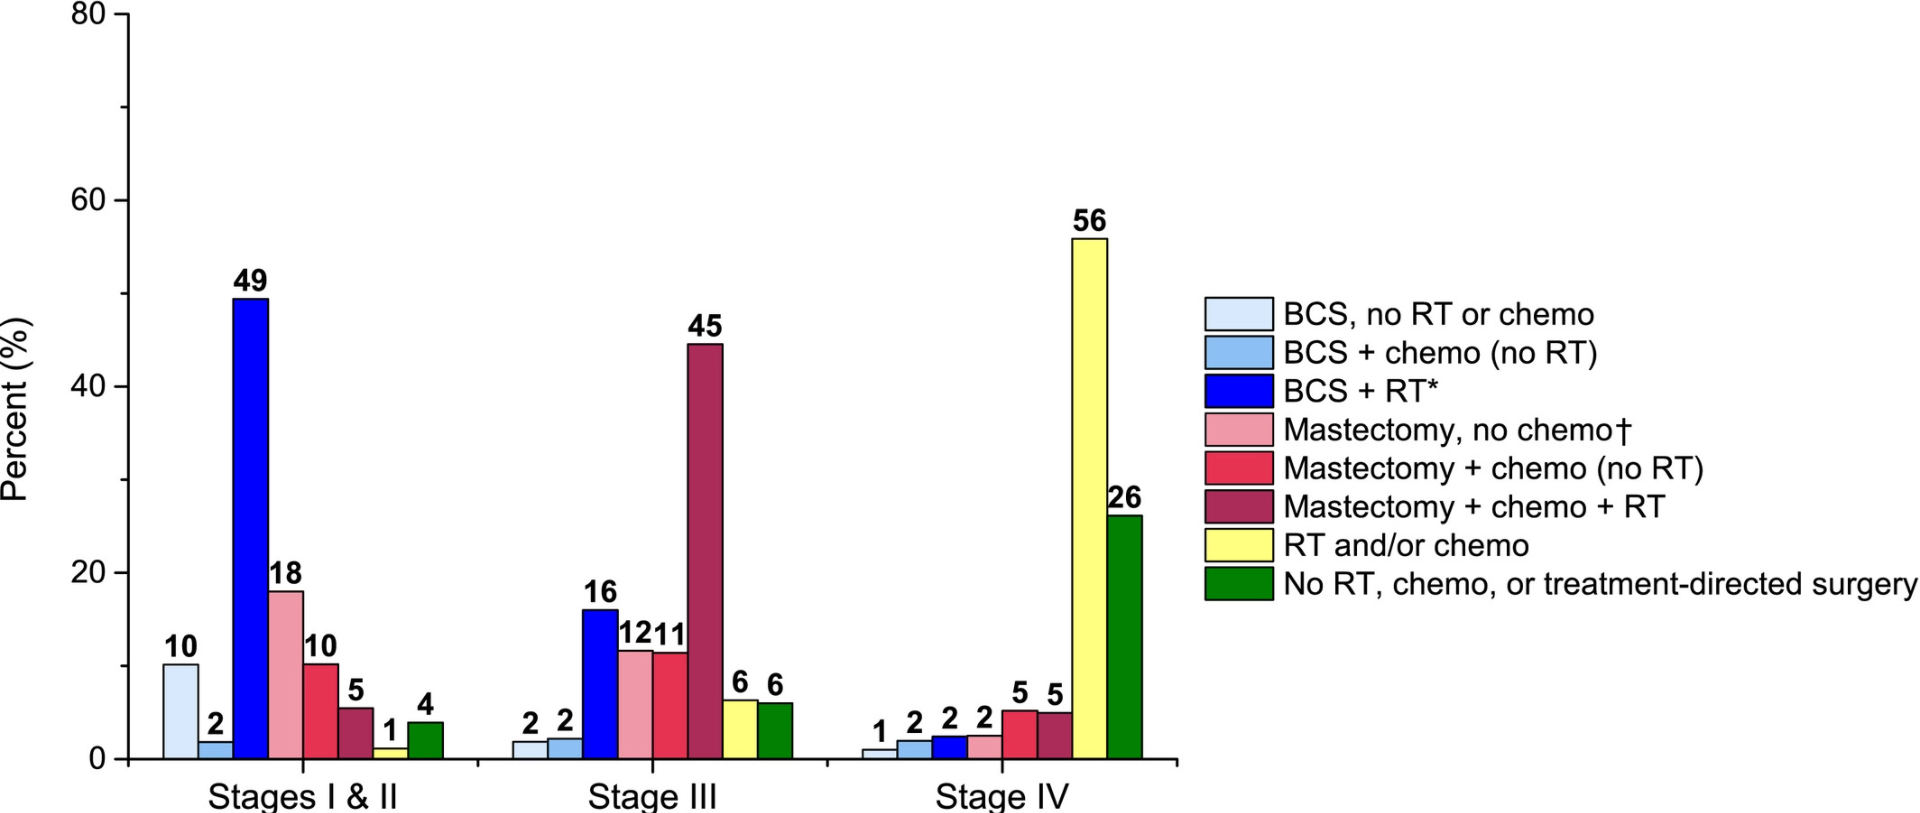
\includegraphics[width=0.7\linewidth]{tumore_seno}
	\caption{Trattamenti per il tumore alla mammella, categoria di neoplasia più diffusa tra la popolazione femminile.\cite{di2021numeri} L'asportazione chirurgica viene adoperata quando il tumore si trova ancora nei suoi stadi iniziali e prende il nome di BCS e mastectomia. Essa è spesso accompagnata da altri trattamenti, come la radioterapia.\cite{miller2019cancer}}
	\label{fig:tumoreseno}
\end{figure}


\subsection*{Radioterapia}

Questa metodologia si avvale di radiazioni ionizzanti per uccidere le cellule neoplastiche e ridurre le dimensioni della massa tumorale. Queste causano dei danni al DNA delle cellule tumorali, che, non essendo in grado di riparare in modo efficiente questi errori, ne impediscono la riproduzione.


\subsection*{Chemioterapia}

Questa tecnica si avvale di alcuni farmaci, detti chemioterapici, che attaccano selettivamente le cellule che si riproducono frequentemente, generalmente impedendo la duplicazione del loro DNA o la separazione di cromosomi appena formati. Per questo motivo i chemioterapici hanno la possibilità di attaccare anche tessuti sani le cui cellule si dividono spesso. 

\begin{figure}[H]
	\centering
	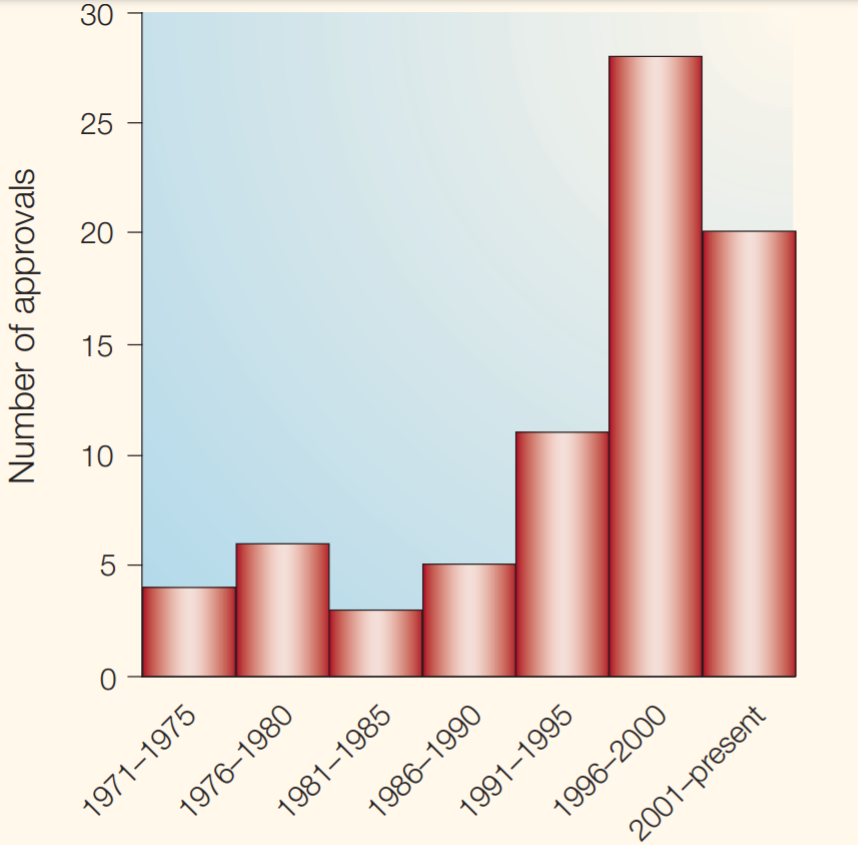
\includegraphics[width=0.5\linewidth]{chemioterapia}
	\caption{Approvazione di nuovi farmaci chemioterapici da parte del FDA. Ciò offre ai malati sia una più vasta scelta di trattamento, sia migliorando la qualità di vita.\cite{chabner2005chemotherapy}}
	\label{fig:chemioterapia}
\end{figure}


\subsection*{Immunoterapia}


L'immunoterapia è una tipologia di trattamento che utilizza componenti del sistema immunitario per eliminare cellule tumorali. Queste strategie che sfruttano le difese immunitarie dello stesso malato sono permettono di attaccare un particolare tipologia di tumore, offrendo, teoricamente, la possibilità di sviluppare una memoria immunologica specifica per le cellule cancerose.\cite{bworld}

\begin{figure}[H]
	\centering
	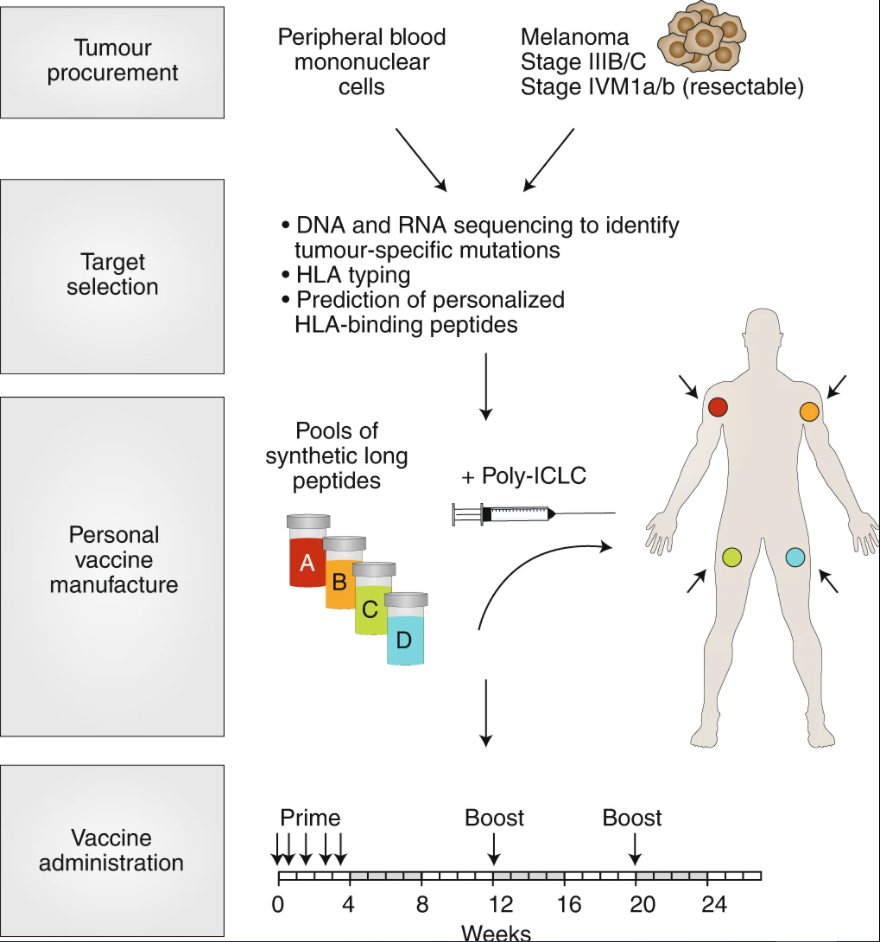
\includegraphics[height=0.2\textheight]{vaccino_cancro}
	\caption{Creazione di vaccini contro il cancro, personalizzato per ogni paziente. Le informazioni ricavate dal confronto di cellule somatiche sane e cancerose sono sfruttate per ottenere un vaccino in grado di sviluppare una reazione immunitaria alle cellule mutate.\cite{scheetz2019engineering}}
	\label{fig:vaccinocancro}
\end{figure}

\newpage

\bibliographystyle{naturemag}
\bibliography{cancro.bib}

\end{document}
